
%% bare_conf.tex
%% V1.4b
%% 2015/08/26
%% by Michael Shell
%% See:
%% http://www.michaelshell.org/
%% for current contact information.
%%
%% This is a skeleton file demonstrating the use of IEEEtran.cls
%% (requires IEEEtran.cls version 1.8b or later) with an IEEE
%% conference paper.
%%
%% Support sites:
%% http://www.michaelshell.org/tex/ieeetran/
%% http://www.ctan.org/pkg/ieeetran
%% and
%% http://www.ieee.org/

%%*************************************************************************
%% Legal Notice:
%% This code is offered as-is without any warranty either expressed or
%% implied; without even the implied warranty of MERCHANTABILITY or
%% FITNESS FOR A PARTICULAR PURPOSE! 
%% User assumes all risk.
%% In no event shall the IEEE or any contributor to this code be liable for
%% any damages or losses, including, but not limited to, incidental,
%% consequential, or any other damages, resulting from the use or misuse
%% of any information contained here.
%%
%% All comments are the opinions of their respective authors and are not
%% necessarily endorsed by the IEEE.
%%
%% This work is distributed under the LaTeX Project Public License (LPPL)
%% ( http://www.latex-project.org/ ) version 1.3, and may be freely used,
%% distributed and modified. A copy of the LPPL, version 1.3, is included
%% in the base LaTeX documentation of all distributions of LaTeX released
%% 2003/12/01 or later.
%% Retain all contribution notices and credits.
%% ** Modified files should be clearly indicated as such, including  **
%% ** renaming them and changing author support contact information. **
%%*************************************************************************


% *** Authors should verify (and, if needed, correct) their LaTeX system  ***
% *** with the testflow diagnostic prior to trusting their LaTeX platform ***
% *** with production work. The IEEE's font choices and paper sizes can   ***
% *** trigger bugs that do not appear when using other class files.       ***                          ***
% The testflow support page is at:
% http://www.michaelshell.org/tex/testflow/



\documentclass[conference]{IEEEtran}
% Some Computer Society conferences also require the compsoc mode option,
% but others use the standard conference format.
%
% If IEEEtran.cls has not been installed into the LaTeX system files,
% manually specify the path to it like:
% \documentclass[conference]{../sty/IEEEtran}





% Some very useful LaTeX packages include:
% (uncomment the ones you want to load)


% *** MISC UTILITY PACKAGES ***
%
%\usepackage{ifpdf}
% Heiko Oberdiek's ifpdf.sty is very useful if you need conditional
% compilation based on whether the output is pdf or dvi.
% usage:
% \ifpdf
%   % pdf code
% \else
%   % dvi code
% \fi
% The latest version of ifpdf.sty can be obtained from:
% http://www.ctan.org/pkg/ifpdf
% Also, note that IEEEtran.cls V1.7 and later provides a builtin
% \ifCLASSINFOpdf conditional that works the same way.
% When switching from latex to pdflatex and vice-versa, the compiler may
% have to be run twice to clear warning/error messages.






% *** CITATION PACKAGES ***
%
%\usepackage{cite}
% cite.sty was written by Donald Arseneau
% V1.6 and later of IEEEtran pre-defines the format of the cite.sty package
% \cite{} output to follow that of the IEEE. Loading the cite package will
% result in citation numbers being automatically sorted and properly
% "compressed/ranged". e.g., [1], [9], [2], [7], [5], [6] without using
% cite.sty will become [1], [2], [5]--[7], [9] using cite.sty. cite.sty's
% \cite will automatically add leading space, if needed. Use cite.sty's
% noadjust option (cite.sty V3.8 and later) if you want to turn this off
% such as if a citation ever needs to be enclosed in parenthesis.
% cite.sty is already installed on most LaTeX systems. Be sure and use
% version 5.0 (2009-03-20) and later if using hyperref.sty.
% The latest version can be obtained at:
% http://www.ctan.org/pkg/cite
% The documentation is contained in the cite.sty file itself.






% *** GRAPHICS RELATED PACKAGES ***
%
\ifCLASSINFOpdf
  % \usepackage[pdftex]{graphicx}
  % declare the path(s) where your graphic files are
  % \graphicspath{{../pdf/}{../jpeg/}}
  % and their extensions so you won't have to specify these with
  % every instance of \includegraphics
  % \DeclareGraphicsExtensions{.pdf,.jpeg,.png}
\else
  % or other class option (dvipsone, dvipdf, if not using dvips). graphicx
  % will default to the driver specified in the system graphics.cfg if no
  % driver is specified.
  % \usepackage[dvips]{graphicx}
  % declare the path(s) where your graphic files are
  % \graphicspath{{../eps/}}
  % and their extensions so you won't have to specify these with
  % every instance of \includegraphics
  % \DeclareGraphicsExtensions{.eps}
\fi
% graphicx was written by David Carlisle and Sebastian Rahtz. It is
% required if you want graphics, photos, etc. graphicx.sty is already
% installed on most LaTeX systems. The latest version and documentation
% can be obtained at: 
% http://www.ctan.org/pkg/graphicx
% Another good source of documentation is "Using Imported Graphics in
% LaTeX2e" by Keith Reckdahl which can be found at:
% http://www.ctan.org/pkg/epslatex
%
% latex, and pdflatex in dvi mode, support graphics in encapsulated
% postscript (.eps) format. pdflatex in pdf mode supports graphics
% in .pdf, .jpeg, .png and .mps (metapost) formats. Users should ensure
% that all non-photo figures use a vector format (.eps, .pdf, .mps) and
% not a bitmapped formats (.jpeg, .png). The IEEE frowns on bitmapped formats
% which can result in "jaggedy"/blurry rendering of lines and letters as
% well as large increases in file sizes.
%
% You can find documentation about the pdfTeX application at:
% http://www.tug.org/applications/pdftex





% *** MATH PACKAGES ***
%
%\usepackage{amsmath}
% A popular package from the American Mathematical Society that provides
% many useful and powerful commands for dealing with mathematics.
%
% Note that the amsmath package sets \interdisplaylinepenalty to 10000
% thus preventing page breaks from occurring within multiline equations. Use:
%\interdisplaylinepenalty=2500
% after loading amsmath to restore such page breaks as IEEEtran.cls normally
% does. amsmath.sty is already installed on most LaTeX systems. The latest
% version and documentation can be obtained at:
% http://www.ctan.org/pkg/amsmath





% *** SPECIALIZED LIST PACKAGES ***
%
%\usepackage{algorithmic}
% algorithmic.sty was written by Peter Williams and Rogerio Brito.
% This package provides an algorithmic environment fo describing algorithms.
% You can use the algorithmic environment in-text or within a figure
% environment to provide for a floating algorithm. Do NOT use the algorithm
% floating environment provided by algorithm.sty (by the same authors) or
% algorithm2e.sty (by Christophe Fiorio) as the IEEE does not use dedicated
% algorithm float types and packages that provide these will not provide
% correct IEEE style captions. The latest version and documentation of
% algorithmic.sty can be obtained at:
% http://www.ctan.org/pkg/algorithms
% Also of interest may be the (relatively newer and more customizable)
% algorithmicx.sty package by Szasz Janos:
% http://www.ctan.org/pkg/algorithmicx




% *** ALIGNMENT PACKAGES ***
%
%\usepackage{array}
% Frank Mittelbach's and David Carlisle's array.sty patches and improves
% the standard LaTeX2e array and tabular environments to provide better
% appearance and additional user controls. As the default LaTeX2e table
% generation code is lacking to the point of almost being broken with
% respect to the quality of the end results, all users are strongly
% advised to use an enhanced (at the very least that provided by array.sty)
% set of table tools. array.sty is already installed on most systems. The
% latest version and documentation can be obtained at:
% http://www.ctan.org/pkg/array


% IEEEtran contains the IEEEeqnarray family of commands that can be used to
% generate multiline equations as well as matrices, tables, etc., of high
% quality.




% *** SUBFIGURE PACKAGES ***
%\ifCLASSOPTIONcompsoc
%  \usepackage[caption=false,font=normalsize,labelfont=sf,textfont=sf]{subfig}
%\else
%  \usepackage[caption=false,font=footnotesize]{subfig}
%\fi
% subfig.sty, written by Steven Douglas Cochran, is the modern replacement
% for subfigure.sty, the latter of which is no longer maintained and is
% incompatible with some LaTeX packages including fixltx2e. However,
% subfig.sty requires and automatically loads Axel Sommerfeldt's caption.sty
% which will override IEEEtran.cls' handling of captions and this will result
% in non-IEEE style figure/table captions. To prevent this problem, be sure
% and invoke subfig.sty's "caption=false" package option (available since
% subfig.sty version 1.3, 2005/06/28) as this is will preserve IEEEtran.cls
% handling of captions.
% Note that the Computer Society format requires a larger sans serif font
% than the serif footnote size font used in traditional IEEE formatting
% and thus the need to invoke different subfig.sty package options depending
% on whether compsoc mode has been enabled.
%
% The latest version and documentation of subfig.sty can be obtained at:
% http://www.ctan.org/pkg/subfig




% *** FLOAT PACKAGES ***
%
%\usepackage{fixltx2e}
% fixltx2e, the successor to the earlier fix2col.sty, was written by
% Frank Mittelbach and David Carlisle. This package corrects a few problems
% in the LaTeX2e kernel, the most notable of which is that in current
% LaTeX2e releases, the ordering of single and double column floats is not
% guaranteed to be preserved. Thus, an unpatched LaTeX2e can allow a
% single column figure to be placed prior to an earlier double column
% figure.
% Be aware that LaTeX2e kernels dated 2015 and later have fixltx2e.sty's
% corrections already built into the system in which case a warning will
% be issued if an attempt is made to load fixltx2e.sty as it is no longer
% needed.
% The latest version and documentation can be found at:
% http://www.ctan.org/pkg/fixltx2e


%\usepackage{stfloats}
% stfloats.sty was written by Sigitas Tolusis. This package gives LaTeX2e
% the ability to do double column floats at the bottom of the page as well
% as the top. (e.g., "\begin{figure*}[!b]" is not normally possible in
% LaTeX2e). It also provides a command:
%\fnbelowfloat
% to enable the placement of footnotes below bottom floats (the standard
% LaTeX2e kernel puts them above bottom floats). This is an invasive package
% which rewrites many portions of the LaTeX2e float routines. It may not work
% with other packages that modify the LaTeX2e float routines. The latest
% version and documentation can be obtained at:
% http://www.ctan.org/pkg/stfloats
% Do not use the stfloats baselinefloat ability as the IEEE does not allow
% \baselineskip to stretch. Authors submitting work to the IEEE should note
% that the IEEE rarely uses double column equations and that authors should try
% to avoid such use. Do not be tempted to use the cuted.sty or midfloat.sty
% packages (also by Sigitas Tolusis) as the IEEE does not format its papers in
% such ways.
% Do not attempt to use stfloats with fixltx2e as they are incompatible.
% Instead, use Morten Hogholm'a dblfloatfix which combines the features
% of both fixltx2e and stfloats:
%
% \usepackage{dblfloatfix}
% The latest version can be found at:
% http://www.ctan.org/pkg/dblfloatfix




% *** PDF, URL AND HYPERLINK PACKAGES ***
%
%\usepackage{url}
% url.sty was written by Donald Arseneau. It provides better support for
% handling and breaking URLs. url.sty is already installed on most LaTeX
% systems. The latest version and documentation can be obtained at:
% http://www.ctan.org/pkg/url
% Basically, \url{my_url_here}.

\usepackage{graphicx}

\graphicspath{{img/}}   % 图片在当前目录下的img目录



% *** Do not adjust lengths that control margins, column widths, etc. ***
% *** Do not use packages that alter fonts (such as pslatex).         ***
% There should be no need to do such things with IEEEtran.cls V1.6 and later.
% (Unless specifically asked to do so by the journal or conference you plan
% to submit to, of course. )


% correct bad hyphenation here
\hyphenation{op-tical net-works semi-conduc-tor}


\begin{document}
%
% paper title
% Titles are generally capitalized except for words such as a, an, and, as,
% at, but, by, for, in, nor, of, on, or, the, to and up, which are usually
% not capitalized unless they are the first or last word of the title.
% Linebreaks \\ can be used within to get better formatting as desired.
% Do not put math or special symbols in the title.
\title{A review on Search-based Software Testing}


% author names and affiliations`
% use a multiple column layout for up to three different
% affiliations
\author{
  \IEEEauthorblockN{Yu Zhang}
  \IEEEauthorblockA{
    Wuhan Texttile University\\
    Student Number: 1815283001\\
    Major: Software Engineering\\
    Instructor: Peng Ye
  }
}

% conference papers do not typically use \thanks and this command
% is locked out in conference mode. If really needed, such as for
% the acknowledgment of grants, issue a \IEEEoverridecommandlockouts
% after \documentclass

% for over three affiliations, or if they all won't fit within the width
% of the page, use this alternative format:
% 
%\author{\IEEEauthorblockN{Michael Shell\IEEEauthorrefmark{1},
%Homer Simpson\IEEEauthorrefmark{2},
%James Kirk\IEEEauthorrefmark{3}, 
%Montgomery Scott\IEEEauthorrefmark{3} and
%Eldon Tyrell\IEEEauthorrefmark{4}}
%\IEEEauthorblockA{\IEEEauthorrefmark{1}School of Electrical and Computer Engineering\\
%Georgia Institute of Technology,
%Atlanta, Georgia 30332--0250\\ Email: see http://www.michaelshell.org/contact.html}
%\IEEEauthorblockA{\IEEEauthorrefmark{2}Twentieth Century Fox, Springfield, USA\\
%Email: homer@thesimpsons.com}
%\IEEEauthorblockA{\IEEEauthorrefmark{3}Starfleet Academy, San Francisco, California 96678-2391\\
%Telephone: (800) 555--1212, Fax: (888) 555--1212}
%\IEEEauthorblockA{\IEEEauthorrefmark{4}Tyrell Inc., 123 Replicant Street, Los Angeles, California 90210--4321}}




% use for special paper notices
%\IEEEspecialpapernotice{(Invited Paper)}




% make the title area
\maketitle

% As a general rule, do not put math, special symbols or citations
% in the abstract
\begin{abstract}
Search Based Software Testing (SBST) formulates
testing as an optimisation problem, which can be attacked using
computational search techniques from the field of Search Based
Software Engineering (SBSE). 

Search Based Software Testing refers to the use of meta-heuristics 
for the optimization of a
task in the context of software testing. Meta-heuristics can solve 
complex problems in which an optimum solution must be found among a 
large amount of possibilities. The use of meta-heuristics in testing
activities is promising because of the high number of inputs that 
should be tested. Previous studies on
search based software testing have focused on the application of 
meta-heuristics for the optimization of
structural and functional criteria. Recently, some researchers have 
proposed the use of SBST for mutation
testing and explored solutions for the cost of application of this 
testing criterion.

Search based mutation testing is a field of interest, however, some 
issues remain unexplored.
For instance, the use of meta-heuristics for the selection of effective 
mutation operators was identified
in only one study. The results have pointed a range of possibilities 
for new studies to be developed, i.e.,
identification of equivalent mutants, experimental studies and application 
to different domains, such as concurrent programs.

Keywords: Search-based Software Testing (SBST), 
Search-based Software Engineering (SBSE), 
meta-heuristics, 
hyper-heuristics, 
Mutation Testing
\end{abstract}

% no keywords




% For peer review papers, you can put extra information on the cover
% page as needed:
% \ifCLASSOPTIONpeerreview
% \begin{center} \bfseries EDICS Category: 3-BBND \end{center}
% \fi
%
% For peerreview papers, this IEEEtran command inserts a page break and
% creates the second title. It will be ignored for other modes.
\IEEEpeerreviewmaketitle



\section{Introduction}

% no \IEEEPARstart
% This demo file is intended to serve as a ``starter file''
% for IEEE conference papers produced under \LaTeX\ using
% IEEEtran.cls version 1.8b and later.
% You must have at least 2 lines in the paragraph with the drop letter
% (should never be an issue)
% I wish you the best of success.

% \hfill mds
 
% \hfill August 26, 2015

% 插入图片
% \LaTeX{} lion---see Fig.\ref{fig-lion}
% \begin{figure}[!t]
%     \centering
%     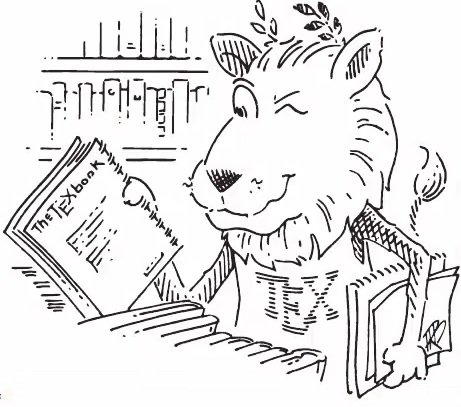
\includegraphics[width=2.5in]{lion.jpg}
%     \caption{\LaTeX\ lion} 
%     \label{fig-lion}
% \end{figure}

% \begin{figure}[!t]
% \centering
% 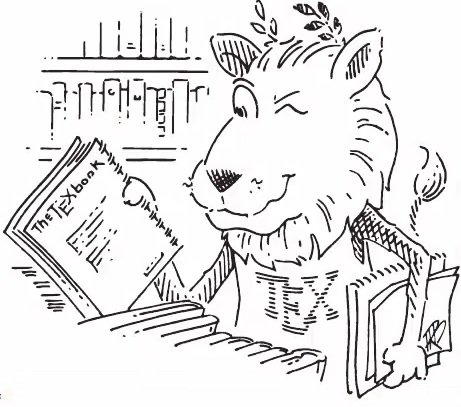
\includegraphics[width=2.5in]{lion.jpg}
% where an .eps filename suffix will be assumed under latex, 
% and a .pdf suffix will be assumed for pdflatex; or what has been declared
% via \DeclareGraphicsExtensions.
% \caption{Simulation results for the network.}
% \label{fig_sim}
% \end{figure}

% An example of a floating figure using the graphicx package.
% Note that \label must occur AFTER (or within) \caption.
% For figures, \caption should occur after the \includegraphics.
% Note that IEEEtran v1.7 and later has special internal code that
% is designed to preserve the operation of \label within \caption
% even when the captionsoff option is in effect. However, because
% of issues like this, it may be the safest practice to put all your
% \label just after \caption rather than within \caption{}.
%
% Reminder: the "draftcls" or "draftclsnofoot", not "draft", class
% option should be used if it is desired that the figures are to be
% displayed while in draft mode.
%
%\begin{figure}[!t]
%\centering
%\includegraphics[width=2.5in]{myfigure}
% where an .eps filename suffix will be assumed under latex, 
% and a .pdf suffix will be assumed for pdflatex; or what has been declared
% via \DeclareGraphicsExtensions.
%\caption{Simulation results for the network.}
%\label{fig_sim}
%\end{figure}

% Note that the IEEE typically puts floats only at the top, even when this
% results in a large percentage of a column being occupied by floats.


% An example of a double column floating figure using two subfigures.
% (The subfig.sty package must be loaded for this to work.)
% The subfigure \label commands are set within each subfloat command,
% and the \label for the overall figure must come after \caption.
% \hfil is used as a separator to get equal spacing.
% Watch out that the combined width of all the subfigures on a 
% line do not exceed the text width or a line break will occur.
%
%\begin{figure*}[!t]
%\centering
%\subfloat[Case I]{\includegraphics[width=2.5in]{box}%
%\label{fig_first_case}}
%\hfil
%\subfloat[Case II]{\includegraphics[width=2.5in]{box}%
%\label{fig_second_case}}
%\caption{Simulation results for the network.}
%\label{fig_sim}
%\end{figure*}
%
% Note that often IEEE papers with subfigures do not employ subfigure
% captions (using the optional argument to \subfloat[]), but instead will
% reference/describe all of them (a), (b), etc., within the main caption.
% Be aware that for subfig.sty to generate the (a), (b), etc., subfigure
% labels, the optional argument to \subfloat must be present. If a
% subcaption is not desired, just leave its contents blank,
% e.g., \subfloat[].


% An example of a floating table. Note that, for IEEE style tables, the
% \caption command should come BEFORE the table and, given that table
% captions serve much like titles, are usually capitalized except for words
% such as a, an, and, as, at, but, by, for, in, nor, of, on, or, the, to
% and up, which are usually not capitalized unless they are the first or
% last word of the caption. Table text will default to \footnotesize as
% the IEEE normally uses this smaller font for tables.
% The \label must come after \caption as always.
%
%\begin{table}[!t]
%% increase table row spacing, adjust to taste
%\renewcommand{\arraystretch}{1.3}
% if using array.sty, it might be a good idea to tweak the value of
% \extrarowheight as needed to properly center the text within the cells
%\caption{An Example of a Table}
%\label{table_example}
%\centering
%% Some packages, such as MDW tools, offer better commands for making tables
%% than the plain LaTeX2e tabular which is used here.
%\begin{tabular}{|c||c|}
%\hline
%One & Two\\
%\hline
%Three & Four\\
%\hline
%\end{tabular}
%\end{table}


% Note that the IEEE does not put floats in the very first column
% - or typically anywhere on the first page for that matter. Also,
% in-text middle ("here") positioning is typically not used, but it
% is allowed and encouraged for Computer Society conferences (but
% not Computer Society journals). Most IEEE journals/conferences use
% top floats exclusively. 
% Note that, LaTeX2e, unlike IEEE journals/conferences, places
% footnotes above bottom floats. This can be corrected via the
% \fnbelowfloat command of the stfloats package.


\subsection{Search-based Software Engineering (SBSE)}

Software Engineering (SE) often considers problems that involve finding a suitable
balance between competing and potentially conflicting goals. There is often a bewilderingly 
large set of choices and finding good solutions can be hard. For instance, the
following is an illustrative list of SE questions \cite{10.1145/2379776.2379787}.

(1) What is the smallest set of test cases that covers all branches in this program?

(2) What is the best way to structure the architecture of this system to enhance its
maintainability?

(3) What is the set of requirements that balances software development cost and 
customer satisfaction?

(4) What is the best allocation of resources to this software development project?

(5) What is the best sequence of refactoring steps to apply to this system?

Answers to these questions might be expected from literature on testing, design,
requirements engineering, SE management, and refactoring, respectively. It might
appear that these questions, which involve different aspects of software engineering,
would be covered by different conferences and specialized journals and would have little
in common. However, all of these questions are essentially optimization questions. As
such, they are typical of the kinds of problem for which SBSE is well adapted and with
which each has been successfully formulated as a search-based optimization problem.
As we shall see in this survey, SBSE has been applied to testing, design, requirements,
project management, and refactoring. This survey will show that work on SBSE applied
to each of these five areas addresses each of the five questions raised before. This
breadth of applicability is one of the enduring appeals of SBSE.

In SBSE, the term “search” is used to refer to the metaheuristic Search-Based 
Optimization (SBO) techniques that are used. SBSE seeks to reformulate SE problems as
SBO problems (or “search problems” for short). The use of the term “search” should not
to be confused with “search” from other contexts such as textual or hypertextual search.
Rather, for SBSE, a search problem is one in which optimal or near-optimal solutions
are sought in a search space of candidate solutions, guided by a fitness function that
distinguishes between better and worse solutions.

The interest in SBO for SE has led to an increased interest in other forms of optimization 
for SE that are not necessarily directly based on a “search”. In the literature
it is common to find the term “SBSE” applied to any form of optimization in which the
problem domain comes from SE and the solution involves optimization according to
some well-defined notion of fitness. In this article, we therefore include classical 
Operations Research (OR) techniques as well as metaheuristic “search-based” techniques
in our understanding of SBSE.

It has been argued that the virtual nature of software makes it well suited for
SBO. This is because fitness is computed directly in terms of the
engineering artifact, without the need for the simulation and modeling inherent in
all other approaches to engineering optimization. The field of SE is also imbued with
rich metrics that can be useful initial candidates for fitness functions. 
This article aims to provide a comprehensive survey of SBSE. It presents
research activity in categories drawn from the ACM subject categories within SE.
For each, it lists the papers, drawing out common themes, such as the type of search
technique used, the fitness definitions, and the nature of evaluation.

A wide range of different optimization and search techniques can and have been used.
The most widely used are local search, Simulated Annealing (SA), Genetic Algorithms
(GAs), Genetic Programming (GP), and Hill Climbing (HC). There is also increasing
evidence of industrial interest in SBSE, with uptake by many software-centric 
organizations including Daimler, Ericsson, IBM, Microsoft, Motorola, Nokia, and NASA.

As the article reveals, 54\% of the overall SBSE literature is concerned with SE
applications relating to testing. There have been several important surveys in this
widely studied general area. For this reason, the present survey will report overall 
trends in the wider SBSE literature(including Search-Based Testing), but it will defer 
to these other three surveys for details on the specific subfield of Search-Based Testing. 
The reader is also referred to an earlier (but considerably longer) version of this 
article that contains a detailed section on testing.

There has been a considerable increase in the quantity of SBSE research over the past
few years (see Figure \ref{fig-increaseInSBSE}). Despite the excellent work in the surveys listed earlier, there
remains, to date, no comprehensive survey of the whole field of study concerning trends
in research. It is therefore timely to review the SBSE literature, the relationships
between the applications to which it has been applied, the techniques used, trends,
and open problems.

\begin{figure}[!t]
    \centering
    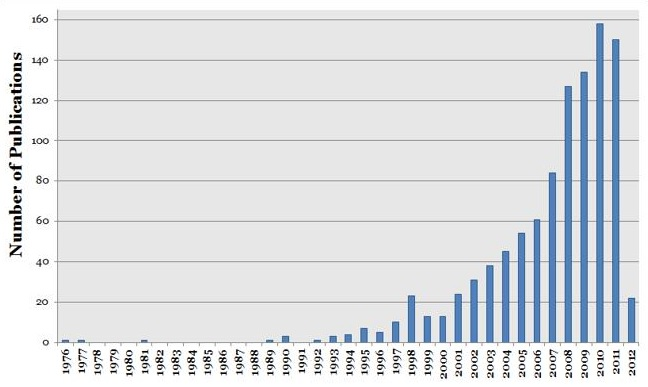
\includegraphics[width=2.5in]{increaseInTheQuantityOfSBSEResearch.jpg}
    \caption{increase in the quantity of SBSE research} 
    \label{fig-increaseInSBSE}
\end{figure}



% Search-based Software Testing (SBST)
\subsection{Search-based Software Testing (SBST)}
Search Based Software Testing (SBST) is the sub-area of
Search Based Software Engineering (SBSE) concerned with
software testing \cite{AFZAL2009957, doi:10.1002/stvr.294}. 
SBSE uses computational search
techniques to tackle software engineering problems (testing
problems in the case of SBST), typified by large complex
search spaces\cite{Mark2010Search}. Test objectives find natural counterparts
as the fitness functions used by SBSE to guide automated
search, thereby facilitating SBSE formulations of many (and
diverse) testing problems. As a result, SBST has proved to
be a widely applicable and effective way of generating test
data, and optimising the testing process. However, there are
many exciting challenges and opportunities that remain open
for further research and development, as we will show in this
paper\cite{7102580}.

It is widely believed that approximately half the budget
spent on software projects is spent on software testing, and
therefore, it is not surprising that perhaps a similar proportion
of papers in the software engineering literature are concerned
with software testing. We report an updated literature analysis
from which we observe that approximately half of all SBSE
papers are SBST papers, a figure little changed since the last
thorough publication audit (for papers up to 2009), which
found 54\% of SBSE papers concerned SBST \cite{10.1145/2379776.2379787}. Many
excellent and detailed surveys of the SBST literature can be
found elsewhere \cite{AFZAL2009957, 5210118, 5210119, doi:10.1002/stvr.294, doi:10.1002/stvr.430}. 
Therefore, rather
than attempting another survey, we provide an analysis of
SBST research trends, focusing on open challenges and areas
for future work and development.

Since the first paper on SBST is also likely to be the first
paper on SBSE, the early history of SBST is also the early
history of SBSE. SBSE is a sub-area of software engineering
with origins stretching back to the 1970s but not formally
established as a field of study in its own right until 2001
, and which only achieved more widespread acceptance
and uptake many years later.

The first mention of software optimisation (of any kind) is
almost certainly due to Ada Augusta Lovelace in 1842. Her
English language translation of the article (written in Italian
by Menabrae), ‘Sketch of the Analytical Engine Invented
by Charles Babbage’ includes seven entries, labelled ‘Note
A’ to ‘Note G’ and initialed ‘A.A.L’. Her notes constituted
an article themselves (and occupied three quarters of the
whole document). In these notes we can see perhaps the first
recognition of the need for software optimisation and source
code analysis and manipulation (a point argued in more detail
elsewhere \cite{5601835}):

“In almost every computation a great variety of
arrangements for the succession of the processes is
possible, and various considerations must influence
the selection amongst them for the purposes of
a Calculating Engine. One essential object is to
choose that arrangement which shall tend to reduce
to a minimum the time necessary for completing the
calculation.” Extract from ‘Note D’.

The introduction of the idea of software testing is probably
due to Turing, who suggested the use of manually
constructed assertions. In his short paper, we can find the
origins of both software testing and software verification. The
first use of optimisation techniques in software testing and
verification probably dates back to the seminal PhD thesis
by James King, who used automated symbolic execution
to capture path conditions, solved using linear programming.
The first formulation of the test input space as a search
space probably dates back seven years earlier to 1962, when
a Cobol test data generation tool was introduced by Sauder. 
Sauder formulates the test generation problem as one
of finding test inputs from a search space, though the search
algorithm is random search, making this likely to be the first
paper on Random Test Data Generation. Sauder’s work is
also significant because it introduces the idea of constraints
to capture path conditions, although these constraints are
manually defined and not automatically constructed.

The first paper to use a meta-heuristic search technique was
probably the work of Boyer, Elspas and Levitt on the SELECT
system \cite{10.1145/800027.808445}. The paper is remarkable in many ways.

Here we can see, not only the first use of computational
search (hill climbing) in software engineering, but also a
hint at the idea (assignment of concrete values) that was
subsequently to become Dynamic Symbolic Execution (DSE). 
Within this single paragraph we therefore may arguably
find the origins of both DSE and SBST (and, by extension,
SBSE too).

The SELECT paper is also remarkable in its sober and
prescient assessment of the relative merits of testing and
verification. Shortly after its publication, these two closely
related research communities entered into a protracted and
unhelpful ‘feud’ that generated a great deal more heat than
light. Fortunately, we have more recently
witnessed an accommodation between the two communities, 
and greater degree of welcome collaboration at their
intersection. We really ought to ruefully reflect on the
delay in this rapprochement given the ‘understanding’ already
set out by the SELECT paper in 1975.

At about the same time2 Miller and Spooner [86], were
also experimenting with optimisation-based approaches for
generating test data (which they refer to as ‘test selection’
in the sense that they ‘select’ from the input space, which,
in the more recent literature we would refer to as ‘test data
generation’).

Unlike Boyer et al., Miller and Spooner used concrete
execution of the program rather than symbolic execution,
making their approach more similar to the techniques that
ultimately became SBST, while the work of Boyer et al.
followed a closely-related (but different) evolutionary path,
which ultimately led to DSE. Current research develops both
these techniques, and also hybrids that combine the best
features of both \cite{6100119, 10.1145/1321631.1321700}.

It appears that SBST research lay dormant for at approximately 
a decade until the work of Korel, which introduced
a practical test data generation approach, the Alternating
Variable Method (AVM), based on hill climbing. The first
use of genetic algorithms for software engineering problems
is usually attributed also to the field of SBST, with the
work of Xanthakis et al., who introduced a genetic
algorithm to develop whole test suites. Subsequent theoretical
and empirical results tend to suggest that AVM outperforms
genetic algorithms (in ‘non-royal road’ test data generation
problems), at least for imperative programs in the C language. 
Since the late 1990s, with a greater overall software
engineering focus on SBSE, there has been an explosion in
SBST publications as the analysis below indicates.

Analysis of Trends in SBST: Figure \ref{fig-increaseInSBST} shows the growth in
papers published on SBST. The data is taken from the SBSE
repository. The aim of the repository is to contain every
SBSE paper, underpinned by regular and careful human-based
update. Although no repository can guarantee 100\% precision
and recall, the SBSE repository has proved sufficiently usable
that it has formed the basis of several other detailed analyses
of the literature, and is widely used by the SBSE
community as a first source of information on related work.
We found a close fit to a quartic function, indicating strong
polynomial growth. If the trend continues, there will be more
than 1,700 SBST papers before the end of this decade.

\begin{figure}[!t]
  \centering
  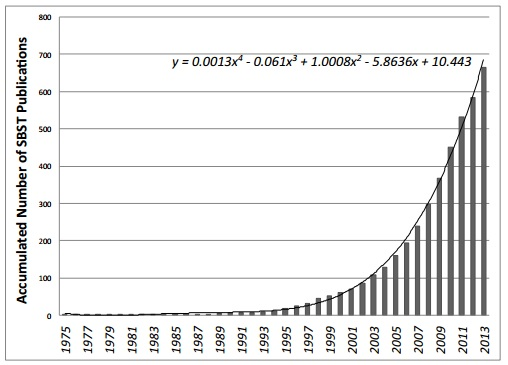
\includegraphics[width=2.5in]{strongHealthOfSBST.jpg}
  \caption{Cumulative number of Search Based Software Testing
  papers. As can be seen, the overall trend continues to suggest
  a polynomial yearly rise in the number of papers, highlighting
  the breadth of interest and strong health of SBST.} 
  \label{fig-increaseInSBST}
\end{figure}


% Meta-heuristics
% \subsection{Meta-heuristics}



% Hyper-heuristics
% \subsection{Hyper-heuristics}





% \subsection{Related works}
% some works here



\section{Conclusion}
% The conclusion goes here.
% \cite{IEEEhowto:kopka}

The future of SBSE is bright. The technology related to SBSE is 
certainly applicable to many fields, but it has not been fully 
considered. In the existing application field, the results have 
been very exciting.

If we think of software engineering as a real engineering discipline, 
then of course we should accept SBSE as a natural result.


% conference papers do not normally have an appendix


% use section* for acknowledgment
\section*{Acknowledgment}


% The authors would like to thank...
Thanks for Professor Ye Peng's guidance and help in the past year. 
Now I have a more comprehensive understanding of software engineering course, 
and I have learned the knowledge that I missed before.


% trigger a \newpage just before the given reference
% number - used to balance the columns on the last page
% adjust value as needed - may need to be readjusted if
% the document is modified later
%\IEEEtriggeratref{8}
% The "triggered" command can be changed if desired:
%\IEEEtriggercmd{\enlargethispage{-5in}}

% references section

% can use a bibliography generated by BibTeX as a .bbl file
% BibTeX documentation can be easily obtained at:
% http://mirror.ctan.org/biblio/bibtex/contrib/doc/
% The IEEEtran BibTeX style support page is at:
% http://www.michaelshell.org/tex/ieeetran/bibtex/
%\bibliographystyle{IEEEtran}
% argument is your BibTeX string definitions and bibliography database(s)
%\bibliography{IEEEabrv,../bib/paper}
%
% <OR> manually copy in the resultant .bbl file
% set second argument of \begin to the number of references
% (used to reserve space for the reference number labels box)

% \begin{thebibliography}{1}

% \bibitem{IEEEhowto:kopka}
% H.~Kopka and P.~W. Daly, \emph{A Guide to \LaTeX}, 3rd~ed.\hskip 1em plus
%   0.5em minus 0.4em\relax Harlow, England: Addison-Wesley, 1999.



% \end{thebibliography}

\bibliographystyle{IEEEtran}
\bibliography{references}

% that's all folks
\end{document}


